Dans l'espace, on considère le cube $ABCDEFGH$ d'arête de longueur égale à 1.

On munit l'espace du repère orthonormé $\left(A;\vect{AB},\vect{AD},\vect{AE}\right)$.

On considère le point $M$ tel que $\vect{BM} = \dfrac{1}{3}\vect{BH}$.

\begin{center}
	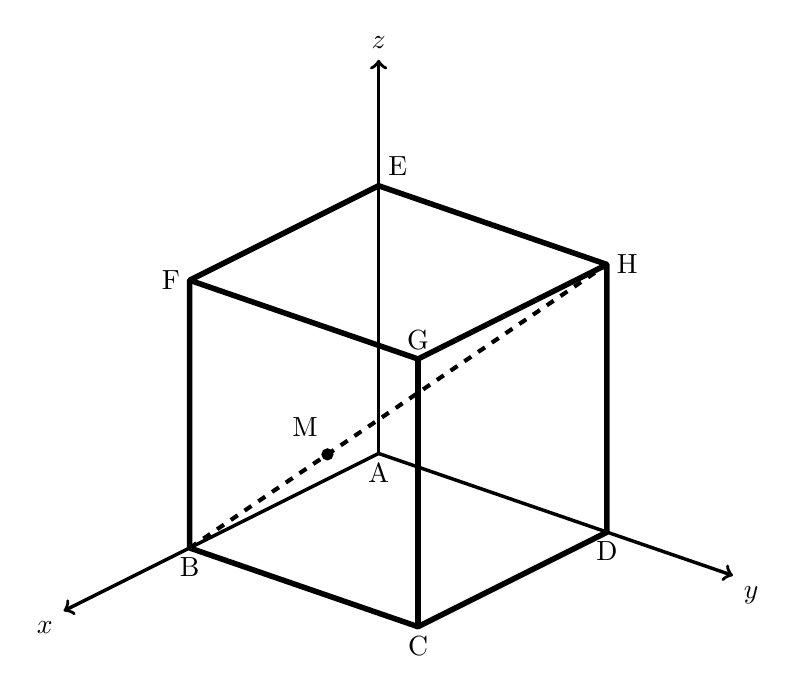
\begin{tikzpicture}
		%axes
		\draw[line width=1.25pt,->] (0,0)--(0,5) node[above] {$z$} ;
		\draw[line width=1.25pt,->] (0,0)--(4.5,-1.55) node[below right] {$y$} ;
		\draw[line width=1.25pt,->] (0,0)--(-4,-2) node[below left] {$x$} ;
		%cube
		\draw[line width=2pt,line join=bevel] (-2.4,-1.2)--(0.5,-2.2)--(2.9,-1)--(2.9,2.4)--(0,3.4)--(-2.4,2.2)--cycle; %BCDHEF
		\draw[line width=2pt,line join=bevel] (-2.4,2.2)--(0.5,1.2)--(2.9,2.4) (0.5,1.2)--(0.5,-2.2) ;%FGH & GC
		%divers
		\draw[dashed,line width=1.5pt] (-2.4,-1.2)--(2.9,2.4) ;
		\filldraw (-0.65,-0.0113) circle[radius=2pt] ;
		%labels
		\foreach \Point/\Nom/\Pos in {(-0.65,0.093)/M/above left,(-2.4,-1.2)/B/below,(0.5,-2.2)/C/below,(2.9,-1)/D/below,(2.9,2.4)/H/right,(0,3.4)/E/above right,(-2.4,2.2)/F/left,(0,0)/A/below,(0.5,1.2)/G/above}%
		\draw \Point node[\Pos] {\Nom} ;
	\end{tikzpicture}
\end{center}

\begin{enumerate}
	\item Par lecture graphique, donner les coordonnées des points $B$, $D$, $E$, $G$ et $H$.
	\item 
	\begin{enumerate}
		\item Quelle est la nature du triangle $EGD$ ? Justifier la réponse.
		\item On admet que l'aire d'un triangle équilatéral de côté $c$ est égale à $\dfrac{\sqrt{3}}{4}c^2$.
		
		Montrer que l'aire du triangle $EGD$ est égale à $\dfrac{\sqrt{3}}{2}$.
	\end{enumerate}
	\item Démontrer que les coordonnées de $M$ sont $\left(\dfrac{2}{3};\dfrac{1}{3}~; ~\dfrac{1}{3}\right)$.
	\item
	\begin{enumerate}
		\item Justifier que le vecteur $\vect{n}(-1;1;1)$ est normal au plan $(EGD)$.
		\item En déduire qu'une équation cartésienne du plan $(EGD)$ est : $- x + y + z - 1 = 0$.
		\item Soit $\mathcal{D}$ la droite orthogonale au plan $(EGD)$ et passant par le point $M$. 
		
		Montrer qu'une représentation paramétrique de cette droite est : \[ \mathcal{D} \: : \: \begin{dcases} x=\dfrac{2}{3} - t \\ y=\dfrac{1}{3} + t \\ z = \dfrac{1}{3} + t \end{dcases},\:t\in\R. \]
	\end{enumerate}
	\item Le cube $ABCDEFGH$ est représenté ci-dessus selon une vue qui permet de mieux percevoir la pyramide $GEDM$, en gris sur la figure :
	
	\begin{center}
		\begin{tikzpicture}[line join=bevel]
			%axes
			\draw[line width=1.25pt,->] (0,0)--(-6,1) node[left] {$y$} ;
			\draw[line width=1.25pt,->] (0,0)--(0,6) node[above] {$y$} ;
			\draw[line width=1.25pt,->] (0,0)--(1.8,2) node[above right] {$x$} ;
			%points
			\tkzDefPoint(0,0){A}\tkzDefPoint(1.2,1.333){B}\tkzDefPoint(-4,0.667){D}\tkzDefPoint(-0.5,2.7){M}
			\begin{scope}[shift=(D)]\tkzDefPoint(1.2,1.333){C}\end{scope}
			\begin{scope}[shift=(A)]\tkzDefPoint(0,4){E}\end{scope}
			\begin{scope}[shift=(D)]\tkzDefPoint(0,4){H}\end{scope}
			\begin{scope}[shift=(C)]\tkzDefPoint(0,4){G}\end{scope}
			\begin{scope}[shift=(B)]\tkzDefPoint(0,4){F}\end{scope}
			%tracés
			\tkzDrawPolygon[lightgray!75,fill=lightgray!75,line width=1pt](D,M,E)
			\tkzDrawPolygon[lightgray,fill=lightgray,line width=1pt](D,G,E)
			\tkzDrawSegments[black,line width=2pt,densely dashed](D,G G,M M,E D,M)
			\tkzDrawSegments[gray,densely dashed,line width=1.75pt](D,C C,B C,G)
			%points&labels&cube
			\tkzDrawPoints[size=4](A,B,C,D,E,F,G,H,M)
			\tkzDrawSegments[black,line width=2pt](D,E E,G)
			\tkzDrawPolygon[gray,line width=1.75pt](A,D,H,E)
			\tkzDrawPolygon[gray,line width=1.75pt](A,B,F,E)
			\tkzDrawPolygon[gray,line width=1.75pt](E,F,G,H)
			\tkzLabelPoints[left](H,G,C)
			\tkzLabelPoints[right](E,F,B)
			\tkzLabelPoints[below](M,D,A)
		\end{tikzpicture}
	\end{center}
	
	Le but de cette question est de calculer le volume de la pyramide $GEDM$.
	
	\begin{enumerate}
		\item Soit K, le pied de la hauteur de la pyramide $GEDM$ issue du point $M$.
		
		Démontrer que les coordonnées du point $K$ sont $\left(\dfrac{1}{3};\dfrac{2}{3};\dfrac{2}{3}\right)$.
		\item En déduire le volume de la pyramide $GEDM$.
		
		\emph{On rappelle que le volume $\mathcal{V}$ d'une pyramide est donné par la formule }
		
		\emph{$\mathcal{V} = \dfrac{b \times h}{3}$ où $b$ désigne l'aire d'une base et $h$ la hauteur associée}.
	\end{enumerate}
\end{enumerate}

